\documentclass[aspectratio=169,10pt]{beamer}

\usepackage{fontspec}
\setmainfont{latinmodern-math.otf}[BoldFont=lmroman10-bold.otf, ItalicFont=lmroman10-italic.otf]
\setsansfont{lmsans10-regular.otf}[BoldFont=lmsans10-bold.otf, ItalicFont=lmsans10-oblique.otf]
\setmonofont{lmmono10-regular.otf}
\usepackage[spanish,es-noquoting]{babel}
\usepackage{booktabs}
\usepackage{graphicx}
\usepackage{xcolor}

\definecolor{utecblue}{HTML}{4C72B0}

\graphicspath{{../reports/figures/}}

\usetheme{default}
\usecolortheme{default}
\setbeamertemplate{navigation symbols}{}
\setbeamertemplate{itemize items}[circle]
\setbeamercolor{structure}{fg=utecblue}
\setbeamercolor{frametitle}{fg=structure}
\setbeamerfont{frametitle}{series=\bfseries,size=\large}
\setbeamertemplate{frametitle}{%
  \vspace{0.6em}\usebeamerfont{frametitle}\usebeamercolor[fg]{frametitle}\insertframetitle\par
  \vspace{-0.3em}{\color{structure}\rule{\textwidth}{0.6pt}}\par\vspace{0.2em}}
\setbeamertemplate{footline}{%
  \hfill\scriptsize\color{gray}\insertframenumber\hspace{1.5em}\vspace{0.8em}}

\definecolor{control}{HTML}{4C72B0}
\definecolor{park}{HTML}{DD8452}
\definecolor{hunt}{HTML}{55A868}
\definecolor{als}{HTML}{C44E52}

\title{\bfseries Dinámica de la marcha para el diagnóstico diferencial de enfermedades neurodegenerativas}
\subtitle{Análisis exploratorio · Entrega P1}
\author{Luis Renato Alvarez Ccopa \quad Andersson Chiroque Silva \\[0.3em] David Teofilo Orihuela Serafin \quad Jeraldine Dione Rojas Vargas}
\institute{Universidad de Ingeniería y Tecnología}
\date{Machine Learning · 2026-1}

\begin{document}

\begin{frame}[plain]
  \titlepage
\end{frame}

\begin{frame}{El problema}
  Tres enfermedades neurodegenerativas destruyen el control motor por mecanismos distintos:

  \vspace{1em}
  \begin{columns}[T]
    \begin{column}{0.32\textwidth}
      \textbf{\color{park}Parkinson}\\[0.3em]
      Degradación de ganglios basales $\rightarrow$ marcha rígida, pasos cortos
    \end{column}
    \begin{column}{0.32\textwidth}
      \textbf{\color{hunt}Huntington}\\[0.3em]
      Movimientos coreicos involuntarios $\rightarrow$ marcha errática
    \end{column}
    \begin{column}{0.32\textwidth}
      \textbf{\color{als}ELA}\\[0.3em]
      Daño a la motoneurona $\rightarrow$ debilidad y compensación
    \end{column}
  \end{columns}

  \vspace{1.5em}
  El diagnóstico diferencial temprano es difícil y descansa en evaluación subjetiva.

  \vspace{0.5em}
  Una marcha instrumentada de 5 minutos es \textbf{barata, no invasiva y repetible}.

  \vspace{1em}
  \begin{block}{Pregunta central}
    ¿La dinámica temporal de la marcha distingue \emph{entre} patologías, o solo separa enfermos de sanos?
  \end{block}
\end{frame}

\begin{frame}{Tarea de Machine Learning}
  \textbf{Clasificación supervisada multiclase}, con el \textbf{sujeto} como unidad de análisis.

  \vspace{1em}
  \begin{columns}[T]
    \begin{column}{0.5\textwidth}
      \begin{itemize}
        \item[\textbf{X}] Descriptores de la serie de intervalos de zancada ($\sim$250 por sujeto)
        \item[\textbf{y}] Control / Parkinson / Huntington / ELA
        \item[\textbf{n}] 64 sujetos
        \item[] Métrica: exactitud balanceada y $F_1$ macro
      \end{itemize}
    \end{column}
    \begin{column}{0.48\textwidth}
      \textbf{Preguntas de investigación}
      \vspace{0.5em}
      \begin{description}
        \item[PI1] ¿Se discrimina entre patologías?
        \item[PI2] ¿Cuánto sesgo introduce evaluar por zancada en vez de por sujeto?
        \item[PI3] ¿Es patología o son confusores (edad, sexo, velocidad)?
      \end{description}
    \end{column}
  \end{columns}
\end{frame}

\begin{frame}{Los datos}
  \textit{Gait in Neurodegenerative Disease Database} — PhysioNet, licencia abierta ODC-By 1.0

  \vspace{0.8em}
  \textbf{Protocolo:} 5 minutos de marcha continua, pasillo de 77 m, resistores de fuerza bajo cada pie, 300 Hz. Los 64 registros son idénticos en duración y muestreo.

  \vspace{1em}
  \begin{columns}[T]
    \begin{column}{0.46\textwidth}
      \textbf{Tres niveles por sujeto}
      \begin{itemize}
        \item Señal cruda de fuerza (90\,000 muestras)
        \item Serie derivada: 13 medidas por zancada
        \item Metadata clínica
      \end{itemize}
      \vspace{0.5em}
      Total: \textbf{15\,160 zancadas}
    \end{column}
    \begin{column}{0.5\textwidth}
      \centering
      \small
      \begin{tabular}{lrrr}
        \toprule
        Grupo & $n$ & Edad & Vel. (m/s) \\
        \midrule
        \color{control}Control    & 16 & 39.3 & 1.35 \\
        \color{park}Parkinson  & 15 & 66.8 & 1.00 \\
        \color{hunt}Huntington & 20 & 46.7 & 1.15 \\
        \color{als}ELA        & 13 & 55.6 & 1.05 \\
        \bottomrule
      \end{tabular}
    \end{column}
  \end{columns}
\end{frame}

\begin{frame}{Hallazgo 1 — La metadata no se puede leer de frente}
  Cuatro defectos que un \texttt{read\_csv} directo no sobrevive:

  \vspace{0.8em}
  \begin{enumerate}
    \item \textbf{Un salto de línea parte un registro.} \texttt{hunt20} está dividido en dos filas $\rightarrow$ el parser devuelve \textbf{65 filas para 64 sujetos}.
      \vspace{0.4em}
    \item \textbf{Los faltantes son la cadena literal \texttt{MISSING}} $\rightarrow$ las columnas dejan silenciosamente de ser numéricas.
      \vspace{0.4em}
    \item \textbf{La variable objetivo declarada está mal.} Los 13 sujetos con ELA tienen \texttt{GROUP = "subjects"} $\rightarrow$ se pierde la clase ELA.
      \vspace{0.4em}
    \item \textbf{Una columna, cuatro escalas incomparables.} Hoehn \& Yahr, capacidad funcional (invertida), meses desde diagnóstico y cero de relleno.
  \end{enumerate}

  \vspace{0.8em}
  \begin{alertblock}{El defecto 4 es una fuga de la variable objetivo}
    El rango de valores identifica el grupo casi perfectamente. La columna queda excluida del modelado.
  \end{alertblock}
\end{frame}

\begin{frame}{Hallazgo 2 — Los grupos no son comparables}
  \centering
  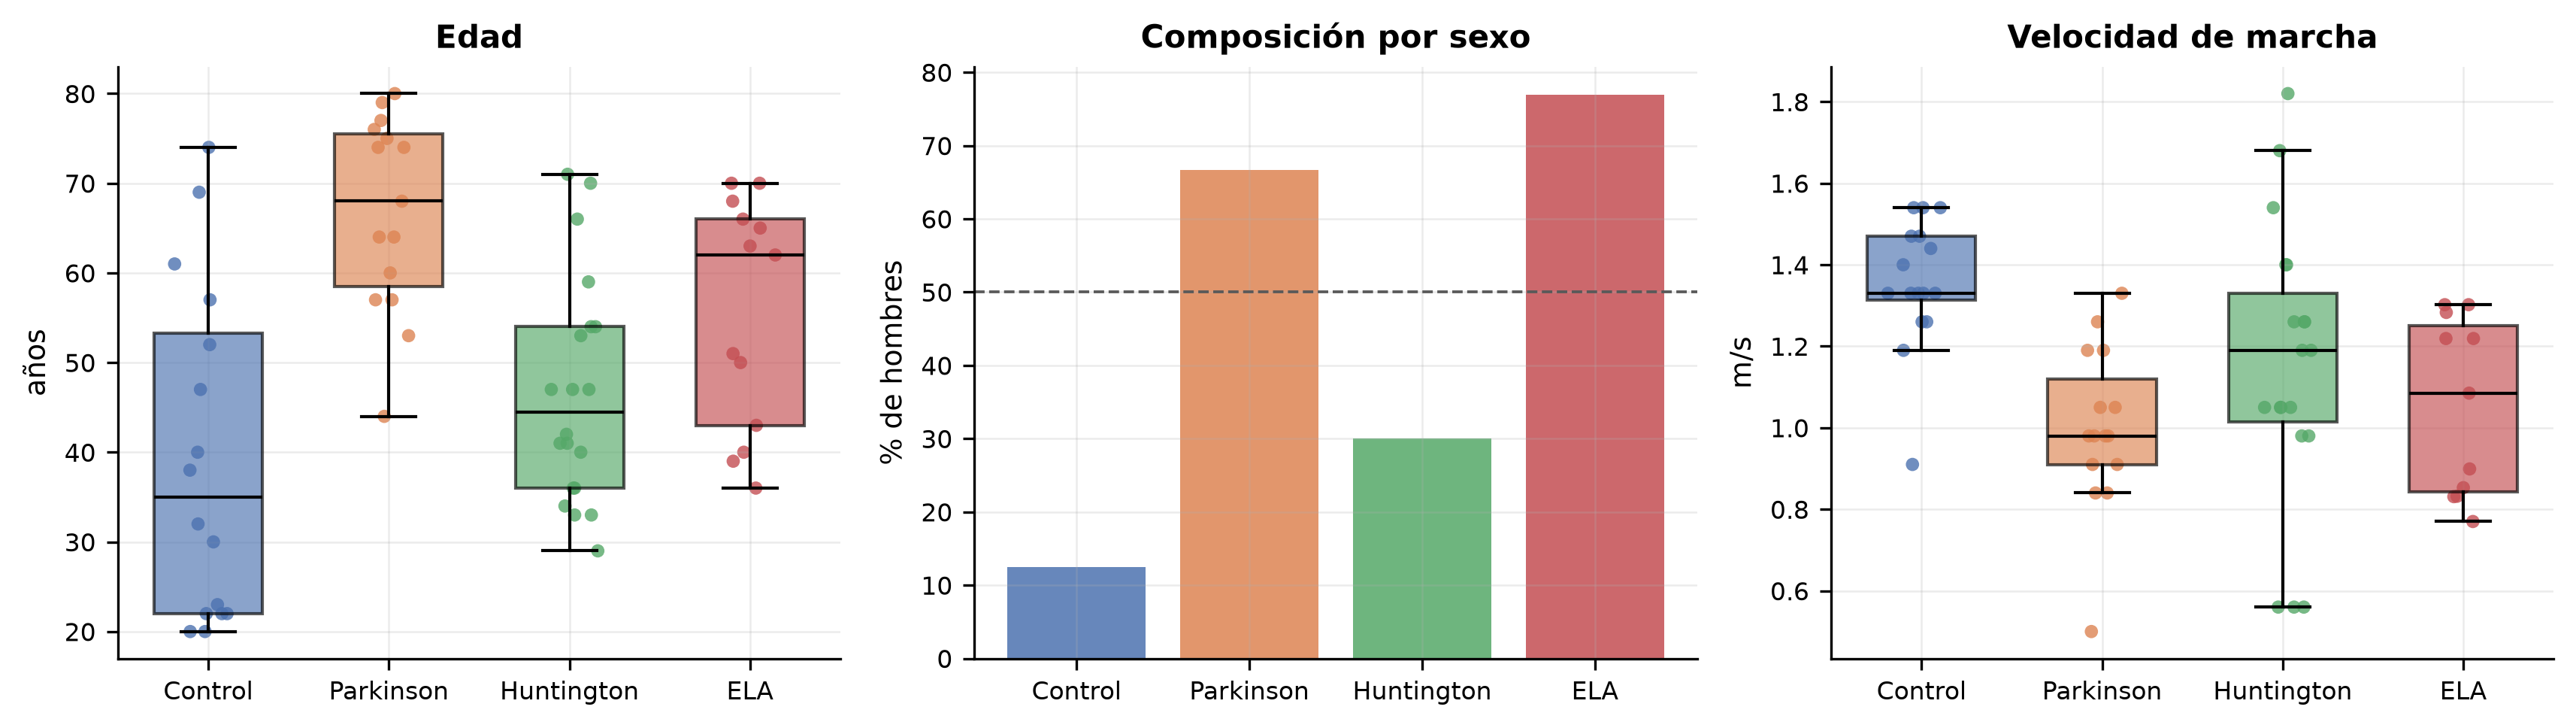
\includegraphics[width=0.92\textwidth]{confusores_demograficos.png}

  \vspace{0.5em}
  \begin{columns}
    \begin{column}{0.33\textwidth}
      \centering \textbf{27 años} de diferencia\\ \small control vs.\ Parkinson
    \end{column}
    \begin{column}{0.33\textwidth}
      \centering \textbf{12.5\% vs.\ 76.9\%}\\ \small de hombres, control vs.\ ELA
    \end{column}
    \begin{column}{0.33\textwidth}
      \centering \textbf{Velocidad}\\ \small es consecuencia, no artefacto
    \end{column}
  \end{columns}
\end{frame}

\begin{frame}{Hallazgo 3 — Un registro inutilizable}
  \texttt{hunt20} viola alguna regla de validez en el \textbf{100\% de sus zancadas}.

  \vspace{1em}
  \centering
  \begin{tabular}{lrr}
    \toprule
    & Pie izquierdo & Pie derecho \\
    \midrule
    Intervalo de zancada mediano & 0.99 s & \textbf{42.9 s} \\
    Fase de apoyo & 61\% & \textbf{98\%} \\
    Fase de balanceo & 39\% & \textbf{2\%} \\
    \midrule
    \multicolumn{3}{l}{Apoyo doble resultante: de $-70\%$ a $+4317\%$ del ciclo} \\
    \bottomrule
  \end{tabular}

  \vspace{1.2em}
  \raggedright
  El canal derecho no registró despegues. Sumado a que su registro empieza 42 s tarde, a que su velocidad es \texttt{MISSING} y a que es el sujeto con la fila partida:

  \vspace{0.5em}
  \centering
  \textbf{falla de cuatro maneras independientes $\rightarrow$ se excluye. Quedan 63 sujetos.}
\end{frame}

\begin{frame}{Hallazgo 4 — El filtrado determina las conclusiones}
  Las series se distribuyen \textbf{sin filtrar} y contienen zancadas de hasta \textbf{55 segundos}.

  \vspace{1em}
  \centering
  \begin{tabular}{lrrr}
    \toprule
    Grupo & CV sin filtrar & CV filtrado & Factor \\
    \midrule
    \color{control}Control    & 0.044 & 0.041 & 1.08 \\
    \color{park}Parkinson  & 0.189 & 0.074 & 2.56 \\
    \color{hunt}Huntington & 0.138 & \textbf{0.105} & 1.32 \\
    \color{als}ELA        & \textbf{0.431} & 0.063 & \textbf{6.80} \\
    \bottomrule
  \end{tabular}

  \vspace{1.2em}
  \raggedright
  Sin filtrar, la ELA aparenta la marcha más inestable: \textbf{10 veces} la variabilidad del control.

  \vspace{0.5em}
  Tras descartar el 5.9\% de zancadas inválidas del grupo, ese CV cae a 0.063.

  \vspace{0.8em}
  \begin{block}{El orden se invierte}
    El grupo más inestable pasa a ser \textbf{\color{hunt}Huntington}, que es lo consistente con la fisiopatología coreica. En este dataset el filtrado no ajusta los resultados: los determina.
  \end{block}
\end{frame}

\begin{frame}{¿Hay señal? (PI1)}
  \centering
  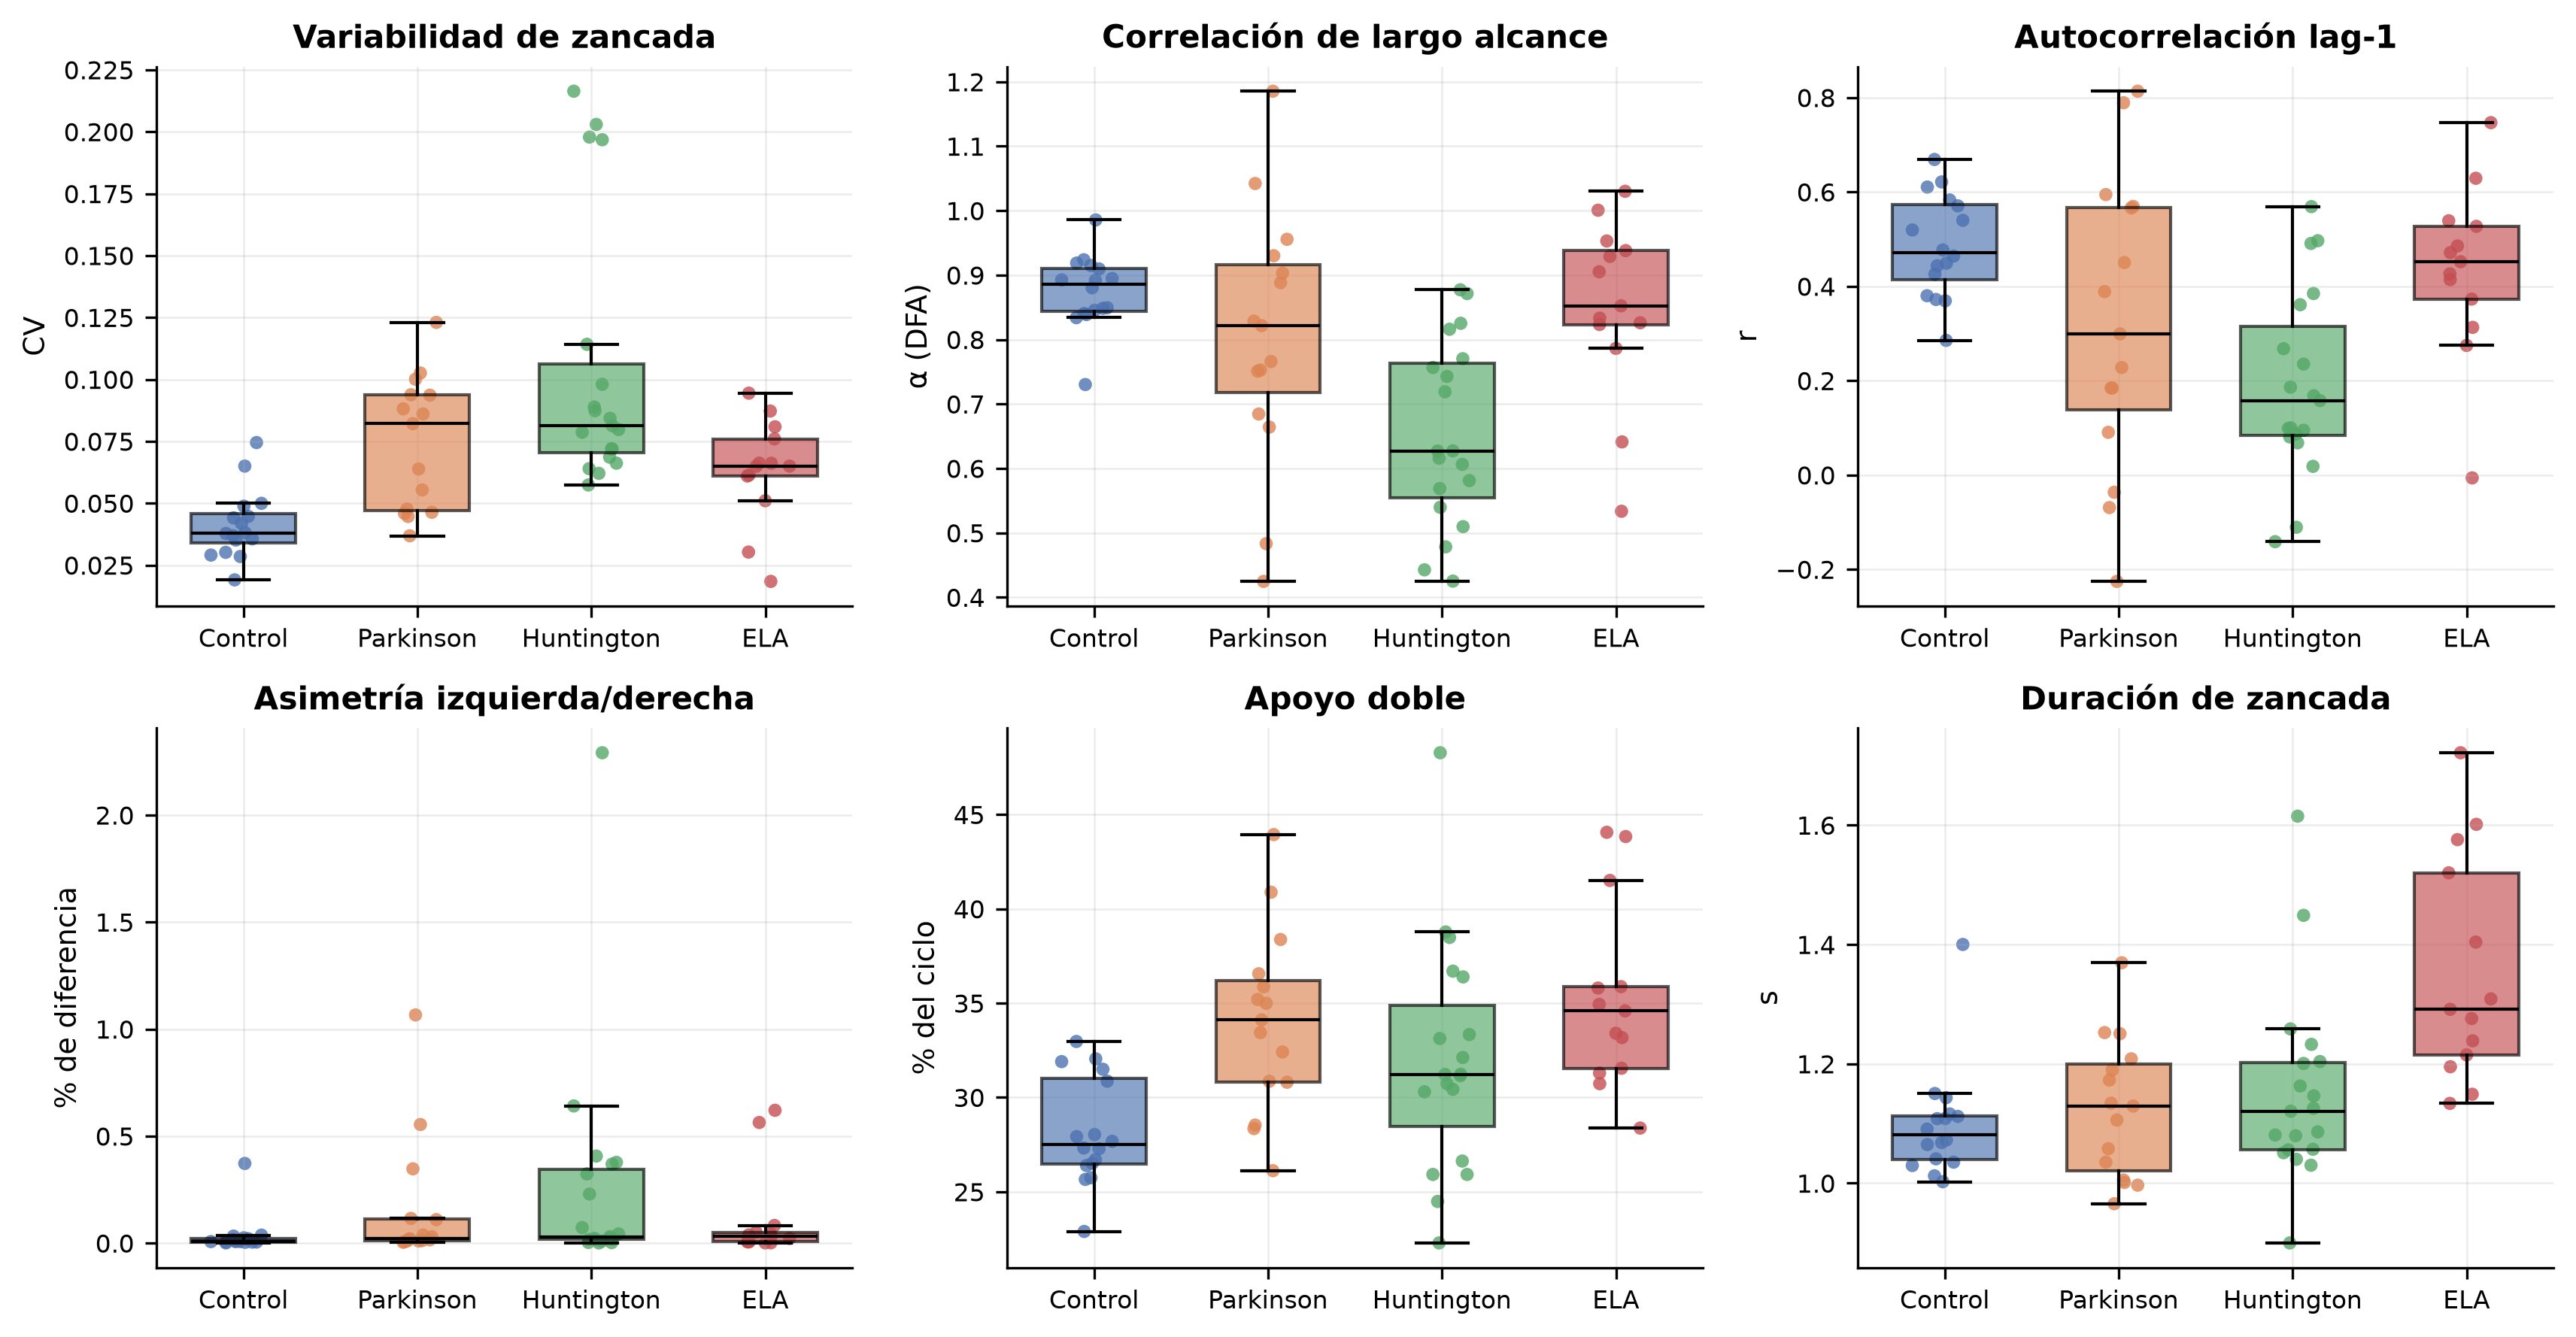
\includegraphics[width=0.78\textwidth]{descriptores_por_grupo.png}

  \vspace{0.4em}
  \raggedright
  \footnotesize
  \textbf{\color{hunt}Huntington} pierde estructura temporal: $\alpha$ de DFA 0.65 vs.\ 0.88 en control; autocorrelación 0.19 vs.\ 0.49. Variable \emph{sin memoria}.\\
  \textbf{\color{als}ELA} compensa: zancada más larga (1.36 s) y más apoyo doble (35\%).\\
  \textbf{\color{park}Parkinson} queda intermedio en casi todo $\rightarrow$ será la clase más difícil.

  \vspace{0.4em}
  \centering
  \small
  Ningún descriptor aislado separa las cuatro clases: la señal es \textbf{multivariada y parcial}.
\end{frame}

\begin{frame}{Hallazgo 5 — Fuga de información por sujeto (PI2)}
  63 sujetos son pocos. La práctica habitual: trocear cada serie en ventanas $\rightarrow$ $\times 8$ filas.

  \vspace{0.5em}
  Pero las ventanas de un sujeto comparten fisiología, calzado y sesión: \textbf{no son independientes}.

  \vspace{1em}
  \centering
  \begin{tabular}{llrr}
    \toprule
    Unidad & Partición & $n$ & Exactitud balanceada \\
    \midrule
    Ventana de 30 zancadas & Aleatoria     & 482 & $0.812 \pm 0.049$ \\
    Ventana de 30 zancadas & Por sujeto    & 482 & $0.622 \pm 0.086$ \\
    Sujeto                 & Estratificada & 63  & $0.642 \pm 0.048$ \\
    \bottomrule
  \end{tabular}

  \vspace{1em}
  \raggedright
  Mismos datos, mismos descriptores, mismo modelo. La única diferencia es la partición.

  \vspace{0.8em}
  \begin{alertblock}{19 puntos porcentuales de optimismo puro}
    La tercera fila es la verificación: evaluar directamente por sujeto da 0.642, que coincide con la estimación agrupada y \emph{no} con la aleatoria. El split agrupado es el estimador correcto.
  \end{alertblock}
\end{frame}

\begin{frame}{La cohorte de validación resuelve el confusor de edad}
  \texttt{gaitpdb}: 165 sujetos con señal (93 Parkinson, 72 control), 16 sensores de fuerza por pie, otro protocolo de captura.

  \vspace{1em}
  \centering
  \begin{tabular}{lrrrr}
    \toprule
    Cohorte & Control & Parkinson & Diferencia & $p$ (Welch) \\
    \midrule
    \texttt{gaitndd} & 39.3 años & 66.8 años & $+27.5$ & $3.2\times10^{-5}$ \\
    \texttt{gaitpdb} & 63.7 años & 66.3 años & $+2.6$  & $0.063$ \\
    \bottomrule
  \end{tabular}

  \vspace{1.2em}
  \raggedright
  El desbalance por sexo también desaparece: 54.8\,\% contra 62.4\,\% de hombres, frente a 12.5\,\% contra 66.7\,\% en la cohorte principal.

  \vspace{0.8em}
  \begin{block}{Deja de ser solo una prueba de generalización}
    Si el eje Parkinson--control se sostiene donde la edad \emph{no} discrimina, la edad no era el mecanismo. Es el instrumento para responder PI3 en P2.
  \end{block}

  \vspace{0.5em}
  \footnotesize
  Sus propios defectos, ya documentados: tabuladores de relleno variables que rompen el parser, talla en centímetros en uno de los tres estudios, un sujeto huérfano con el ID mal escrito, y Hoehn \& Yahr y UPDRS como fuga perfecta de la etiqueta.
\end{frame}

\begin{frame}{Limitaciones (PI3)}
  \begin{itemize}
    \item \textbf{Confusores no corregibles \emph{dentro de} la cohorte principal.} El grupo control es 27 años más joven y mayoritariamente femenino. La cohorte externa acota el efecto, pero solo para el eje Parkinson--control: Huntington y ELA quedan sin contraparte pareada.
      \vspace{0.6em}
    \item \textbf{Muestra reducida.} 63 sujetos obligan a validación \textit{leave-one-subject-out} e intervalos de confianza amplios.
      \vspace{0.6em}
    \item \textbf{El filtrado es diferencial por clase.} Elimina 260 zancadas en Huntington y 1 en control. Queda abierto si una zancada de 3 s es error del sensor o congelamiento real.
      \vspace{0.6em}
    \item \textbf{Talla y peso no son comparables} entre cohortes: se recolectaron por separado y con convenciones de unidades distintas.
  \end{itemize}
\end{frame}

\begin{frame}{Siguientes pasos — P2}
  \begin{enumerate}
    \item \textbf{Protocolo de evaluación:} validación agrupada por sujeto (LOSO), búsqueda de hiperparámetros \emph{anidada}, intervalos de confianza por bootstrap.
      \vspace{0.5em}
    \item \textbf{Baselines:} clase mayoritaria y un baseline clínico que use \emph{solo} la velocidad de marcha. Si los descriptores de dinámica no lo superan, no justifican su complejidad.
      \vspace{0.5em}
    \item \textbf{Modelos:} regresión logística multinomial regularizada, ensamble de árboles y una CNN 1D sobre la serie cruda.
      \vspace{0.5em}
    \item \textbf{Validación externa y control del confusor:} entrenar y evaluar el eje Parkinson–control por separado en la cohorte confundida y en la pareada; la diferencia acota el efecto demográfico. Más regresión de severidad UPDRS dentro del grupo de pacientes.
      \vspace{0.5em}
    \item \textbf{Análisis de confusores:} reentrenar en subgrupos comparables por edad y medir la pérdida.
      \vspace{0.5em}
    \item \textbf{Interpretación:} importancia por permutación agrupada y matriz de confusión, con foco en Parkinson–ELA.
  \end{enumerate}
\end{frame}

\begin{frame}[plain]
  \vfill
  \centering
  {\Large\bfseries\color{structure} Gracias}

  \vspace{1.5em}
  \begin{tabular}{rl}
    Datos & PhysioNet \texttt{gaitndd} y \texttt{gaitpdb} (ODC-By 1.0) \\
    Código & repositorio público del proyecto \\
  \end{tabular}
  \vfill
\end{frame}

\end{document}
